\usetikzlibrary{arrows.meta}
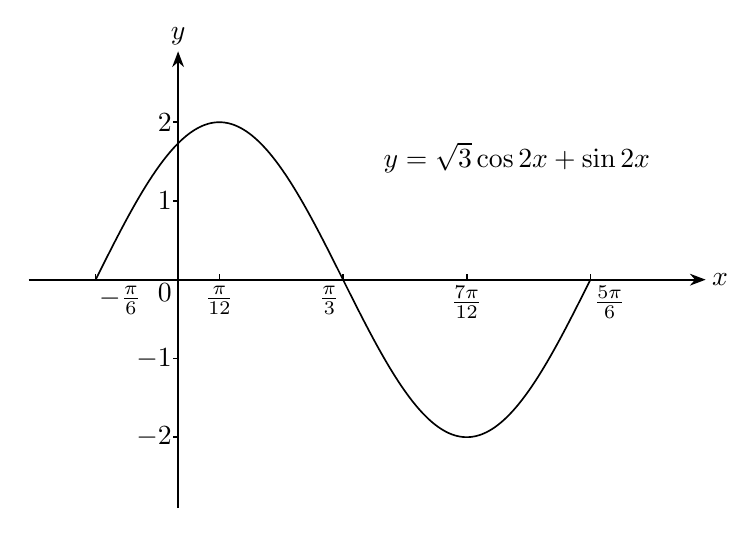
\begin{tikzpicture}[x=2cm,y=1cm,line width=.6pt,>=Stealth,font=\normalsize]
% axes: math x in radians, physical x=2cm/rad, y=1cm/unit
\draw[->] (-0.95,0)--(3.35,0) node[right,inner sep=0pt,xshift=2pt] {$x$};
\draw[->] (0,-2.9)--(0,2.9) node[above,inner sep=0pt,yshift=2pt] {$y$};
% x ticks
\foreach \xp/\lab in {-0.5236/$-\frac{\pi}{6}$,0.2618/$\frac{\pi}{12}$,1.0472/$\frac{\pi}{3}$,1.8326/$\frac{7\pi}{12}$,2.6180/$\frac{5\pi}{6}$} {\draw[line width=.6pt] (\xp,0)--(\xp,0.07);}
% labels below with side offsets to avoid diagonal zero-crossings
\node[anchor=north west,inner sep=0pt,yshift=-2pt,xshift=1pt] at (-0.5236,0) {$-\frac{\pi}{6}$};
\node[anchor=north,inner sep=0pt,yshift=-2pt] at (0.2618,0) {$\frac{\pi}{12}$};
\node[anchor=north east,inner sep=0pt,yshift=-2pt,xshift=-1pt] at (1.0472,0) {$\frac{\pi}{3}$};
\node[anchor=north,inner sep=0pt,yshift=-2pt] at (1.8326,0) {$\frac{7\pi}{12}$};
\node[anchor=north west,inner sep=0pt,yshift=-2pt,xshift=1pt] at (2.6180,0) {$\frac{5\pi}{6}$};
\node[anchor=north east,inner sep=0pt,xshift=-2pt,yshift=-1pt] at (0,0) {$0$};
% y ticks
\foreach \yp/\lab in {1/$1$,2/$2$,-1/$-1$,-2/$-2$} {\draw[line width=.6pt] (0,\yp)--(-0.035,\yp);}
\node[anchor=east,inner sep=0pt,xshift=-2pt] at (0,2) {$2$};
\node[anchor=east,inner sep=0pt,xshift=-2pt] at (0,1) {$1$};
\node[anchor=east,inner sep=0pt,xshift=-2pt] at (0,-1) {$-1$};
\node[anchor=east,inner sep=0pt,xshift=-2pt] at (0,-2) {$-2$};
% curve y=2*sin(2x+pi/3), PGF angles in degrees
\draw[domain=-0.5236:2.6180,samples=220] plot (\x,{2*sin(2*deg(\x)+60)});
% formula label in whitespace above curve
\node[anchor=west,inner sep=0pt] at (1.30,1.55) {$y=\sqrt{3}\cos 2x+\sin 2x$};
\end{tikzpicture}
